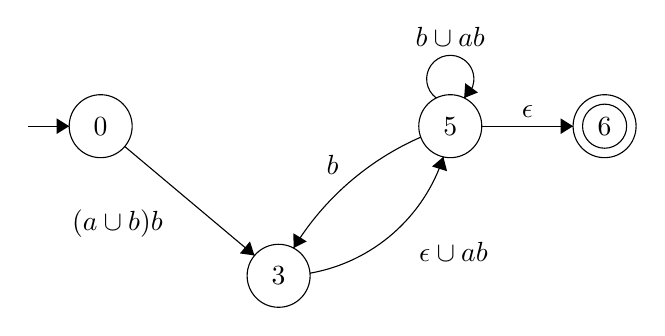
\begin{tikzpicture}[scale=0.2]
    \tikzstyle{every node}+=[inner sep=0pt]
    \draw [black] (4.8,-6.9) circle (2);
    \draw (4.8,-6.9) node {$0$};
    \draw [black] (16.1,-16.4) circle (2);
    \draw (16.1,-16.4) node {$3$};
    \draw [black] (27,-6.9) circle (2);
    \draw (27,-6.9) node {$5$};
    \draw [black] (36.8,-6.9) circle (2);
    \draw (36.8,-6.9) node {$6$};
    \draw [black] (36.8,-6.9) circle (1.4);
    \draw [black] (0.2,-6.9) -- (2.8,-6.9);
    \fill [black] (2.8,-6.9) -- (2,-6.4) -- (2,-7.4);
    \draw [black] (26.565,-8.849) arc (-17.84573:-80.00609:10.888);
    \fill [black] (26.56,-8.85) -- (25.84,-9.46) -- (26.8,-9.76);
    \draw (27.2,-14.21) node [below] {$\epsilon\cup ab$};
    \draw [black] (29,-6.9) -- (34.8,-6.9);
    \fill [black] (34.8,-6.9) -- (34,-6.4) -- (34,-7.4);
    \draw (31.9,-6.4) node [above] {$\epsilon$};
    \draw [black] (26.118,-5.114) arc (234:-54:1.5);
    \draw (27,-1.9) node [above] {$b\cup ab$};
    \fill [black] (27.88,-5.11) -- (28.76,-4.76) -- (27.95,-4.17);
    \draw [black] (17.047,-14.639) arc (148.53091:113.61727:17.864);
    \fill [black] (17.05,-14.64) -- (17.89,-14.22) -- (17.04,-13.7);
    \draw (19.53,-10.01) node [above] {$b$};
    \draw [black] (6.33,-8.19) -- (14.57,-15.11);
    \fill [black] (14.57,-15.11) -- (14.28,-14.22) -- (13.64,-14.98);
    \draw (5.86,-12.14) node [below] {$(a\cup b)b$};
    \end{tikzpicture}